\documentclass[12pt,a4paper]{ctexart}
\usepackage[final]{pdfpages}
\setCJKmainfont{SimSun}[AutoFakeBold,AutoFakeSlant]
\setmainfont{TeX Gyre Termes}
\linespread{1.5}
\ctexset {
section = {
name = {第,章},
number = \chinese{section},
},
subsection = {
name = {第,节},
number = \chinese{subsection},
}
}
\date{}




\title{\Huge\textbf{2023年全国大学生信息安全竞赛\\作品报告}}
\begin{document}
\maketitle
\vspace{6cm}
{
    \Large\textbf{作品名称}:\textbf{\underline{\makebox[10cm]{基于TrustZone-M函数级内存地址}}}

    \textbf{\underline{\makebox[13cm]{空间随机化的可信实时系统}}}

    \textbf{电子邮箱}:\underline{\makebox[10cm]{\textbf{213211377@seu.edu.cn}}}

    \textbf{提交时间}:\underline{\makebox[10cm]{\textbf{\today}}}
}
\thispagestyle{empty}
\clearpage
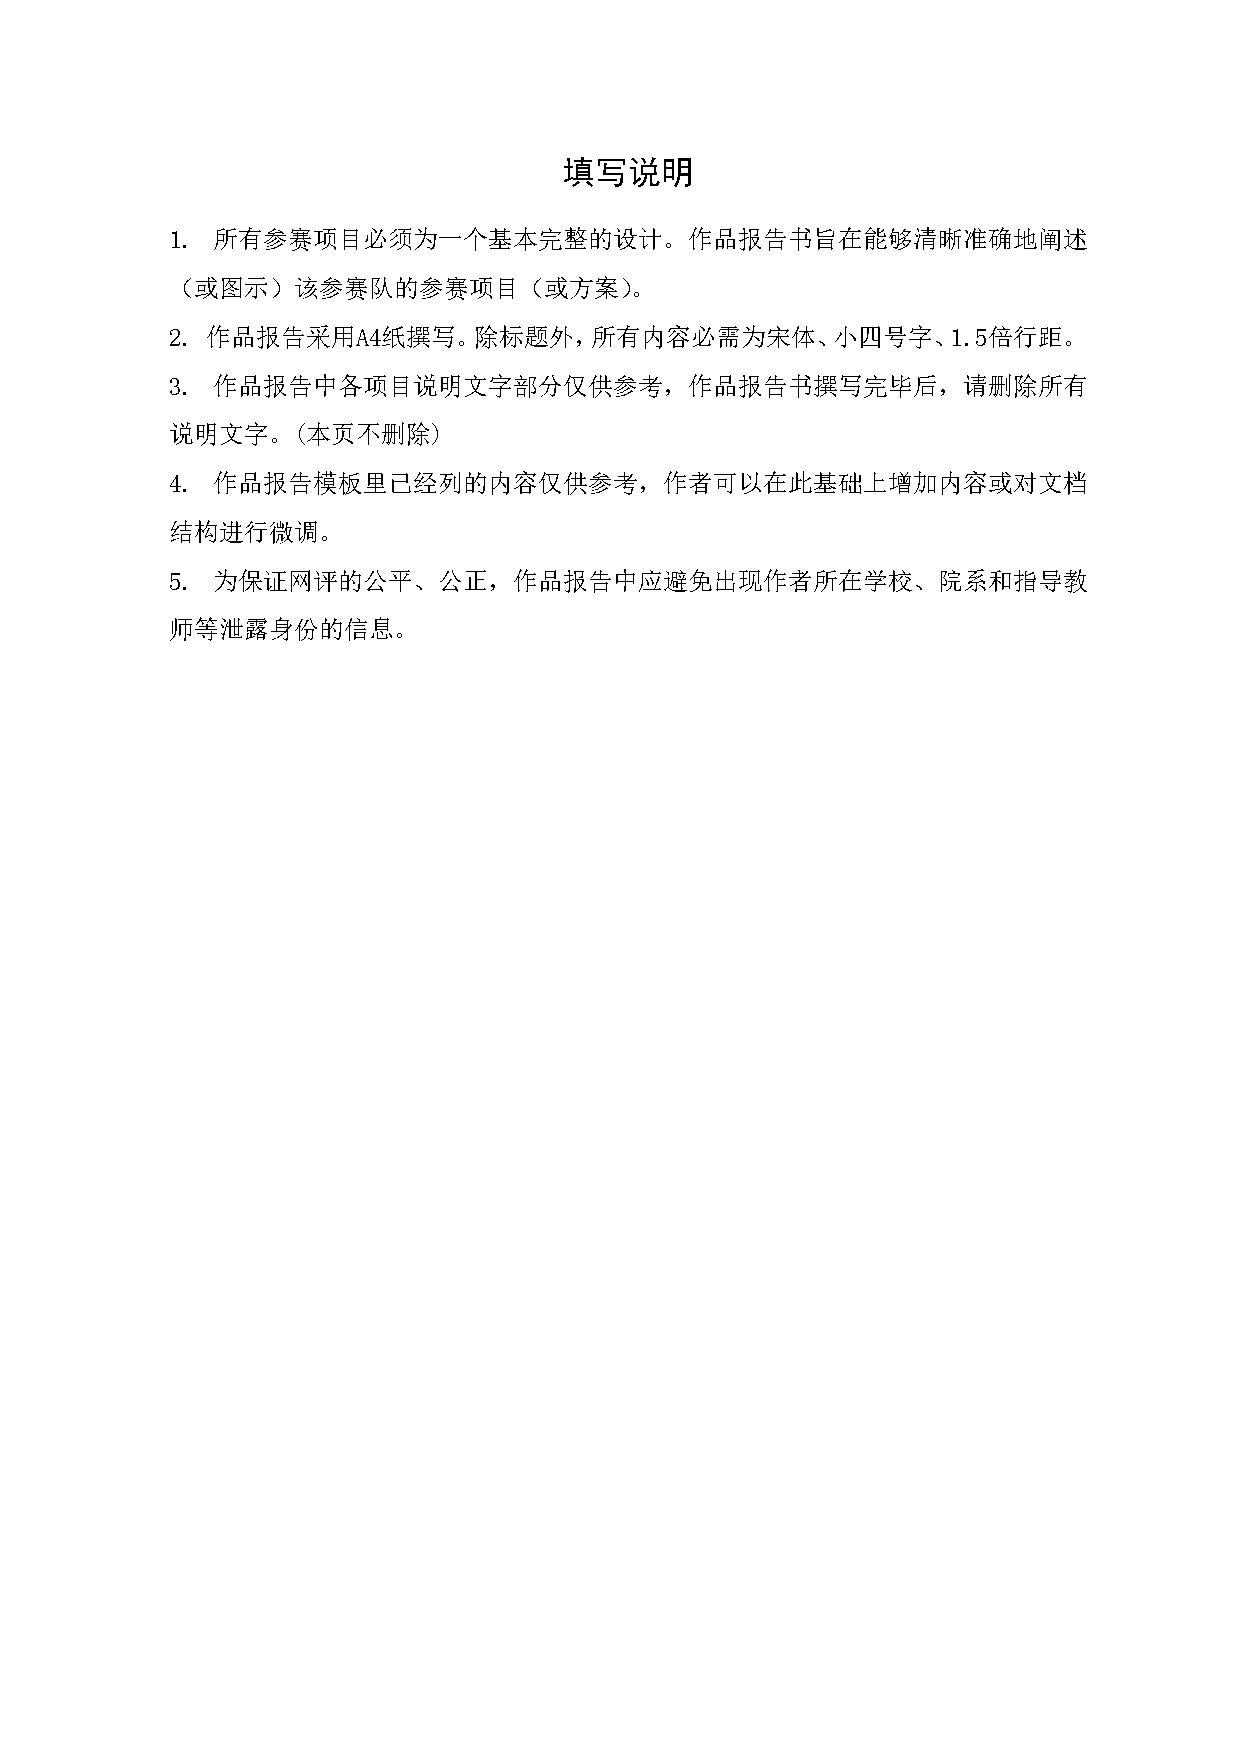
\includepdf{src/request.pdf}
\thispagestyle{empty}
\clearpage
\tableofcontents
\thispagestyle{empty}
\clearpage
\setcounter{page}{1}
\section*{摘要}
\addcontentsline{toc}{section}{摘要}
简要说明创作本作品之动机、功能、特性、创新处、实用性等
\section{作品概述}
可包括背景分析、研究现状、特色描述、应用前景分析等
\section{作品设计与实现}
可包括系统架构设计、系统实现方案、系统实现功能等
\section{作品测试与分析}
可包括测试方案、测试环境搭建、测试数据及分析等
\section{创新性说明}
\section{总结}
\end{document}